\documentclass[../main.tex]{subfiles}

\begin{document}

\chapter{Об’єктно-орієнтоване проектування ІС}

\section{Архітектурне проектування}

При створенні програмних систем перед розробниками часто постає проблема вибору тих чи інших проектних рішень. У цих випадках на допомогу приходять патерни. Справа в тому, що майже напевно подібні завдання вже вирішувалися раніше і вже існують добре продумані елегантні рішення, складені експертами. Якщо ці рішення описати і систематизувати в каталоги, то вони стануть доступними менш досвідченим розробникам, які після вивчення зможуть використовувати їх як шаблони або зразки для вирішення завдань подібного класу. Патерни якраз описують рішення таких завдань, що повторюються.

Концепція створення програмного забезпечення з використанням патернів, безсумнівно, дуже важлива, але відносно молода, можливо, тому до цих пір немає чіткого визначення, що ж таке патерн. Про це свідчать безперервні дискусії в популярній літературі і на відповідних форумах в мережі.

Наприклад, чи слід вважати алгоритми і структури даних паттернами? З цього питання існують протилежні думки. Відповідно до одного з них, алгоритми є обчислювальними паттернами, а добре відома фундаментальна монографія Дональда Кнута "Мистецтво програмування"\ по суті являє собою каталог таких патернів. Згідно з іншим думку, алгоритми не є паттернами, так як можуть бути вирішені ними проблеми занадто малі (оперують такими поняттями як обчислювальна складність і споживання ресурсів), а область рішення добре окреслена. Патерни ж вирішують проблеми більшого масштабу, при цьому патерн дає не~конкретне рішення, а якийсь шлях до вирішення, причому, вибір правильного патерну — завдання нетривіальне, що припускає від архітектора наявність інтуїції, досвіду, певного творчості.

% TODO one more problem with special sense of quotes " and "  -- spaces after the quotes may go away; backslash solves the problem, but I still recommend to change all quotes to `` and '' or \enqoute{...} or maybe << and >>

В силу популярності каталогу GoF \cite{gof} часто під паттернами проектування мають на увазі всі види патернів програмної індустрії, що є не зовсім коректним. В області розробки програмних систем існує безліч паттернів, які відрізняються областю застосування, масштабом, вмістом, стилем опису. Наприклад, в залежності від сфери застосування існують такі патерни як патерни аналізу, проектування, тестування, документування, організації процесу розробки, планування проектів та інші.

В даний час найбільш популярними паттернами є патерни проектування. Однією з поширених класифікацій таких патернів є класифікація за ступенем деталізації і рівню абстракції розглянутих систем. Згідно \cite{pattern_oriented_arch}, патерни проектування програмних систем діляться на наступні категорії:

\begin{enumerate}
	\item Архітектурні паттерни.
	\item Патерни проектування.
	\item Ідіоми.
\end{enumerate}

Архітектурні патерни, будучи найбільш високорівневими паттернами, описують структурну схему програмної системи в цілому. В даній схемі вказуються окремі функціональні складові системи, звані підсистемами, а також взаємини між ними. Прикладом архітектурного патерну є добре відома програмна парадигма "модель-уявлення-контролер"\ (model-view-controller — MVC).

У свою чергу, підсистеми можуть складатися з архітектурних одиниць рівнем нижче. Патерни проектування описують схеми деталізації програмних підсистем і відносин між ними, при цьому вони не впливають на структуру програмної системи в цілому і зберігають незалежність від реалізації мови програмування. Патерни GoF відносяться саме до цієї категорії. Згідно \cite{gof}, під паттернами проектування об'єктно-орієнтованих систем розуміється опис взаємодії об'єктів і класів, адаптованих для вирішення загальної задачі проектування в конкретному контексті.

Ідіоми, будучи низькорівневими паттернами, мають справу з питаннями реалізації будь-якої проблеми з урахуванням особливостей даної мови програмування. При цьому часто одні й ті ж ідіоми для різних мов програмування виглядають по-різному або не мають сенсу зовсім. Наприклад, в C++ для усунення можливих втрат пам'яті можуть використовуватися інтелектуальні покажчики. Інтелектуальний покажчик містить покажчик на ділянку динамічно виділеної пам'яті, який буде автоматично звільнений при виході із зони видимості. У середовищі Java такої проблеми просто не існує, так як там використовується автоматичне прибирання сміття. Зазвичай, для використання ідіом потрібно глибоко знати особливості застосовуваної мови програмування.

Слід зазначити, що в програмній області існують і інші види патернів, що не відносяться до проектування взагалі, наприклад, патерни аналізу, тестування, документування та ін.

Завдання кожного патерну — дати чіткий опис проблеми та її рішення у відповідній області. Для цього можуть використовуватися різні формати описів від художньо-описового \cite{pattern_language} до суворого, академічного \cite{gof}. У~загальному випадку опис паттерна завжди містить такі елементи:

\begin{enumerate}
	\item Назву патерну. Являє собою унікальне смислове ім'я, що однозначно визначає цю задачу або проблему і її рішення.
	\item Задачу, котру потрібно вирішити. Тут дається розуміння того, чому розв'язувана проблема дійсно є такою, чітко описує її межі.
	\item Рішення. Тут вказується, як саме таке рішення пов'язане з проблемою, наводиться шляхи її вирішення.
	\item Результати використання патерну. Зазвичай наводяться переваги, недоліки і компроміси.
\end{enumerate}

Один зі співавторів GoF, Джон Вліссідес \cite{patterns_application} наводить такі переваги застосування патернів проектування:

\begin{enumerate}
	\item Вони (патерни) дозволяють підсумувати досвід експертів і зробити його доступним рядовим розробникам.
	\item Імена патернів утворюють свого роду словник, який дозволяє розробникам краще розуміти один одного.
	\item Якщо в документації системи зазначено, які патерни в ній використовуються, це дозволяє читачеві швидше зрозуміти систему.
	\item Патерни спрощують реструктуризацію системи незалежно від того, чи використовувалися патерни при її проектуванні.
\end{enumerate}

Правильно обрані патерни проектування дозволяють зробити програмну систему більш гнучкою, її легше підтримувати і модифікувати, а код такої системи в більшій мірі відповідає концепції повторного використання.

\subsection{Діаграми пакетів}

Як зображено на діаграмі \ref{server_packages}, серверна частина складається з таких пакетів:
\begin{itemize}
	\item \enquote{api} — містить основний код серверної частини;
	\begin{itemize}
		\item \enquote{controllers} — містить код обробників запитів до серверу;
		\item \enquote{helpers} — містить код компонентів, що використовуються різними обробниками;
		\begin{itemize}
			\item \enquote{sql} — містить код компонентів для роботи з реляційною БД;
		\end{itemize}
		\item \enquote{swagger} — містить код компонентів, що використовуються різними обробниками;
	\end{itemize}
	\item \enquote{config} — містить конфігураційні файли;
	\item \enquote{test} — містить тести серверної частини.
\end{itemize}

\begin{figure}[H]
	\centering
	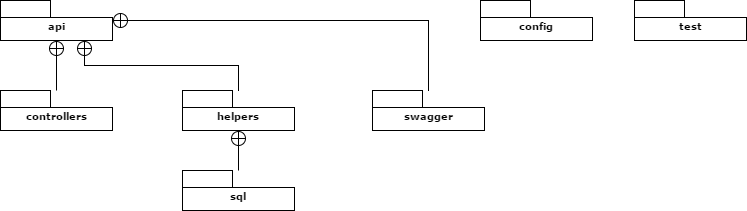
\includegraphics[width=0.75\textwidth]{3_backend_packages}
	\caption{Діаграма пакетів серверної частини}
	\label{server_packages}
\end{figure}


Діаграма \ref{client_packages} показує структуру пакетів клієнтського Android додатку. Він складається з таких пакетів:
\begin{itemize}
	\item \enquote{api} — містить опис інтерфейсу взаємодії з серверною частиною;
	\item \enquote{bundlers} — містить опис серіалізаторів нестандартних типів;
	\item \enquote{events} — містить опис подій, на яких базується взаємодія в додатку;
	\item \enquote{models} — містить опис моделей даних;
	\item \enquote{prefs} — містить опис користувацьких налаштувань;
	\item \enquote{screens} — містить опис екранів додатку;
	\begin{itemize}
		\item \enquote{base} — містить опис базових класів сущностей користувацького інтерфейсу;
	\end{itemize}
	\item \enquote{utils} — містить код утилітарних класів;
	\item \enquote{adapters} — містить опис адаптерів для різноманітних списків;
	\item \enquote{di} — містить опис класів, потрібних для реалізації ін'єкції залежностей;
	\item \enquote{ui} — містить опис класів, що використовуються для побудови користувацького інтерфейсу.
\end{itemize}

\begin{figure}[H]
	\centering
	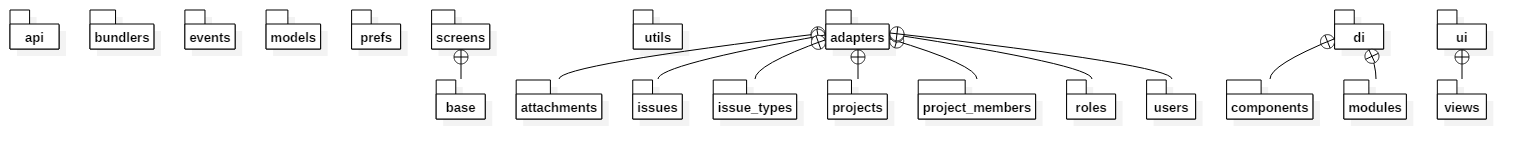
\includegraphics[width=1\textwidth]{3_package_structure_client}
	\caption{Діаграма пакетів Android клієнту}
	\label{client_packages}
\end{figure}

\subsection{Діаграми компонентів}

Точкою входу клієнтського додатку є клас \enquote{App}. Для того, щоб система могла створити його екземпляр та запустити додаток за допомогою нього, він унаслідуваний від системного класу \enquote{Application} та заздалегідь прописаний в \enquote{AndroidManifest.xml}. Кожна активність в додатку є наслідуваною від класу \enquote{BaseActivity}. Таким чином досягається розповсюдження базової логіки на кожну конкретну активність. Для відображення списків в коді передбачено класи, іменовані у стилі \enquote{<Назва списку>Adapter} та \enquote{<Назва списку>Item}. Таким чином, забезпечується інкапсуляція даних щодо кожного елементу списку та конвертації даних цього елементу в звичний для користувача візуальний вигляд. Детальніше, структура комнонентів зображена на діаграмі \ref{client_components}.

\begin{figure}[H]
	\centering
	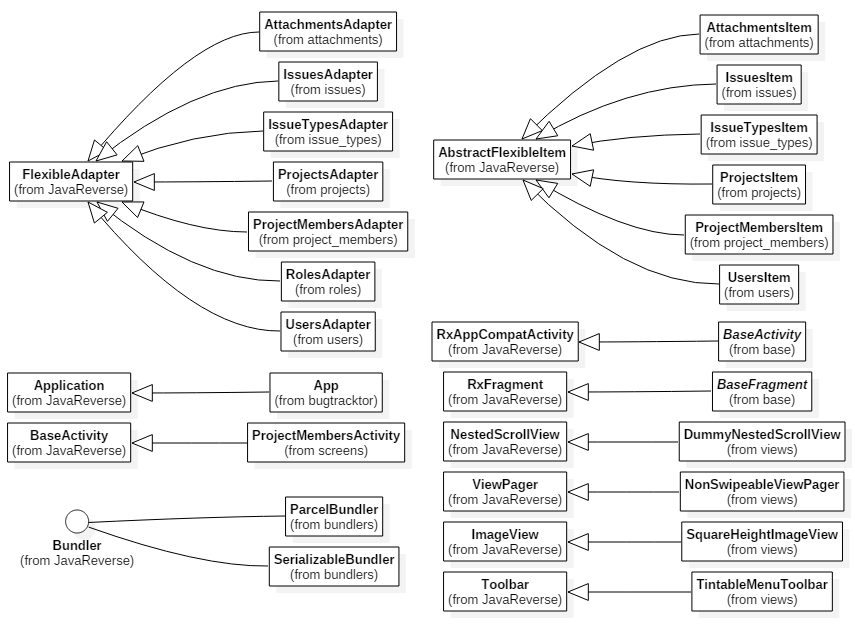
\includegraphics[height=0.9\textheight]{3_hierarchy_client}
	\caption{Діаграма компонентів Android клієнту}
	\label{client_components}
\end{figure}

\section{Детальне проектування}

Для детального проектування серверної частини було застосовано Swagger — фреймворк для опису специфікації REST API. Наявність опису API такого формату є додатковою основою стабільності остаточного продукту, оскільки він дозволяє командам, що працюють над різними частинами системи, знати всі необхідні для взаємодії з сервером дані ще до того, як сервер введений у дію. Опис API за допомогою Swagger передбачає опис наявних моделей даних та доступних REST ресурсів. Діаграма \ref{available_rest_resources} відображає результат проектування за допомогою Swagger.

\begin{figure}[H]
	\centering
	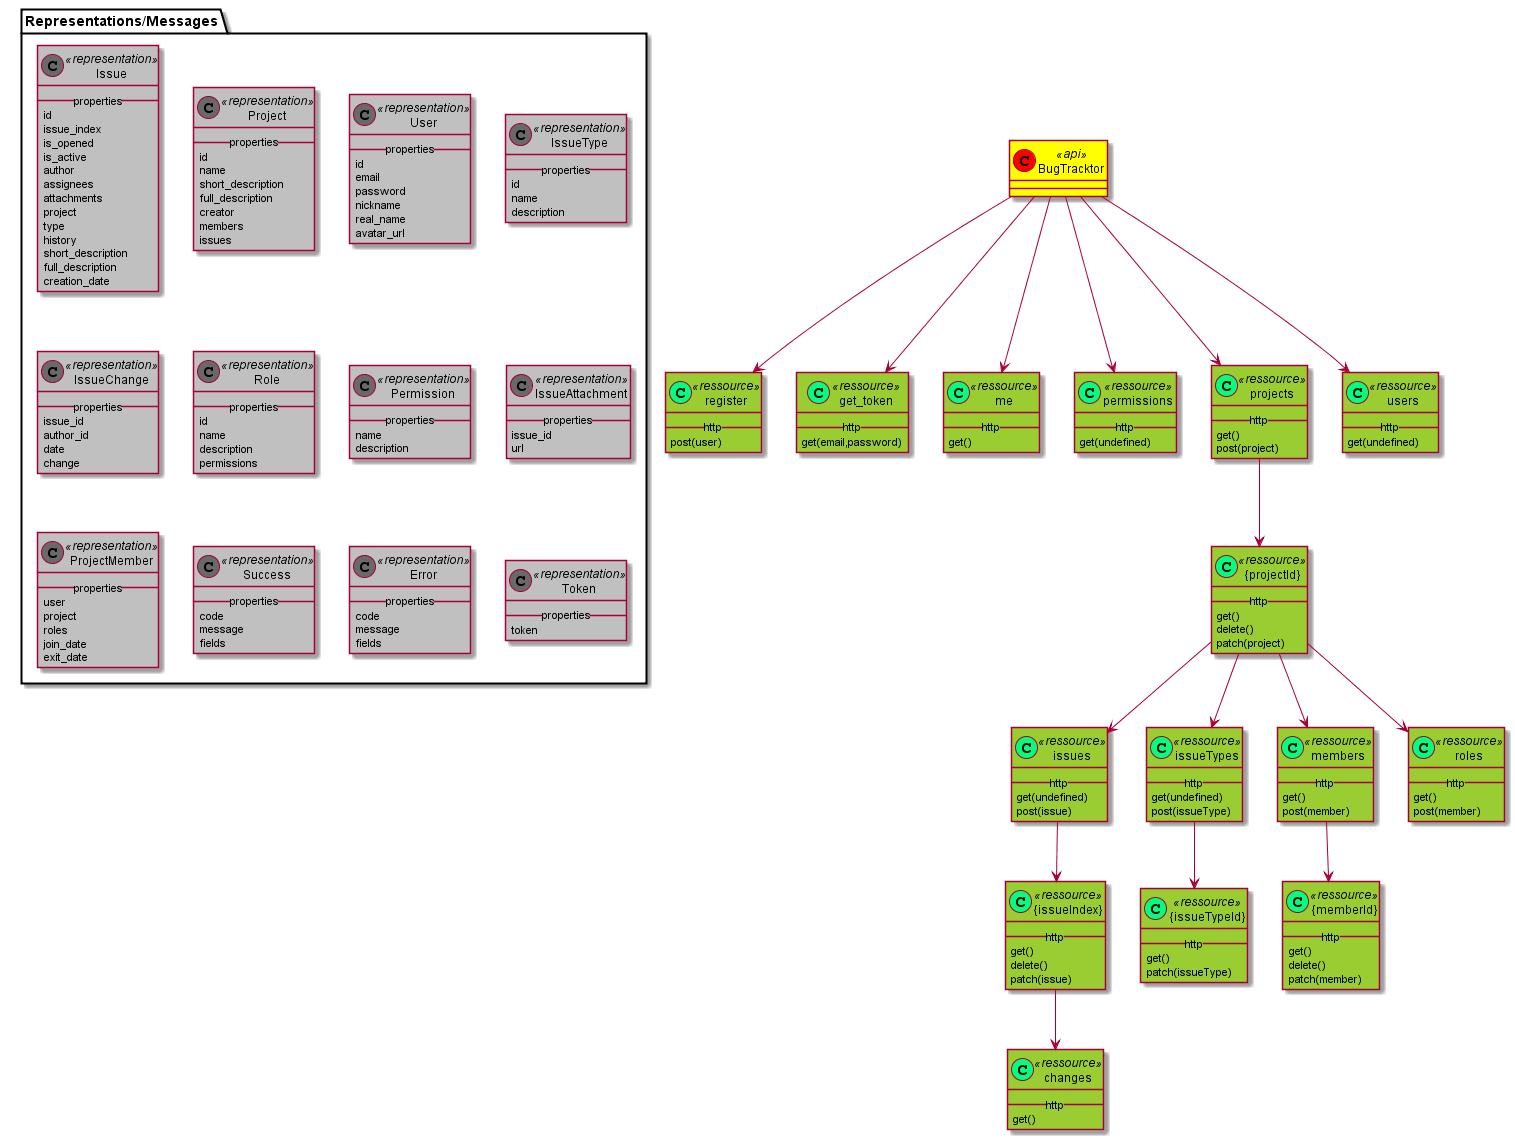
\includegraphics[width=1\textwidth]{3_diagram_rest_api}
	\caption{Діаграма наявних REST ресурсів веб-серверу}
	\label{available_rest_resources}
\end{figure}

Використання Swagger дозволяє візуально оцінити необхідні методи взаємодії з серверною частиною (див. рис. \ref{available_rest_endpoints}).

\begin{figure}[H]
	\centering
	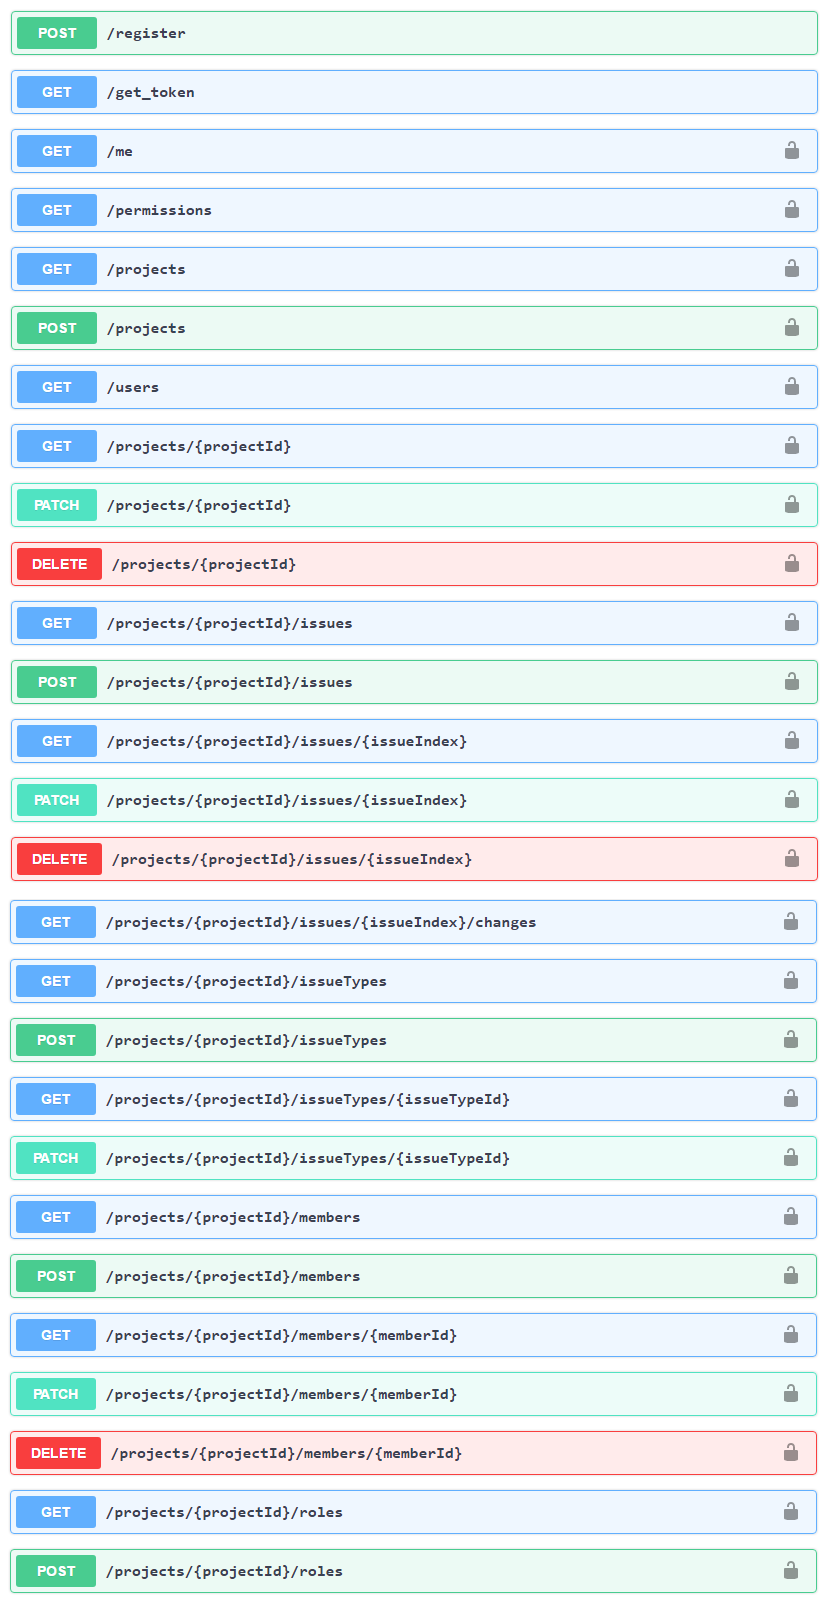
\includegraphics[width=0.75\textwidth]{3_backend_endpoints}
	\caption{Список необхідних методів взаємодії з сервером}
	\label{available_rest_endpoints}
\end{figure}

Кожен з методів взаємодії має один з чотирьох типів: GET, POST, PATCH або DELETE. Якщо для взаємодії потрібен URI параметр, то його повинно бути вказано на місці тексту, обрамленого фігурними скобками. Наявність іконки \enquote{замку} в описі методу взаємодії свідчить про необхідність авторизації для його використання.

Завдяки наявності специфікації взаємодії з сервером, існує можливість генерації моделей даних для різних платформ, в тому числі і для мобільних додатків. Таким чином, моделі даних можуть бути згенеровані для клієнтського додатку, що спрощує імплементацію взаємодії з сервером. Тому, моделі даних для Android клієнту матимуть вигляд, представлений на діаграмі \ref{client_models}.

% TODO мне кажется что стОит долить какой-то воды (малополезного текста) чтоб не получалось аж такого огромного вертикального отступа

\begin{figure}[H]
	\centering
	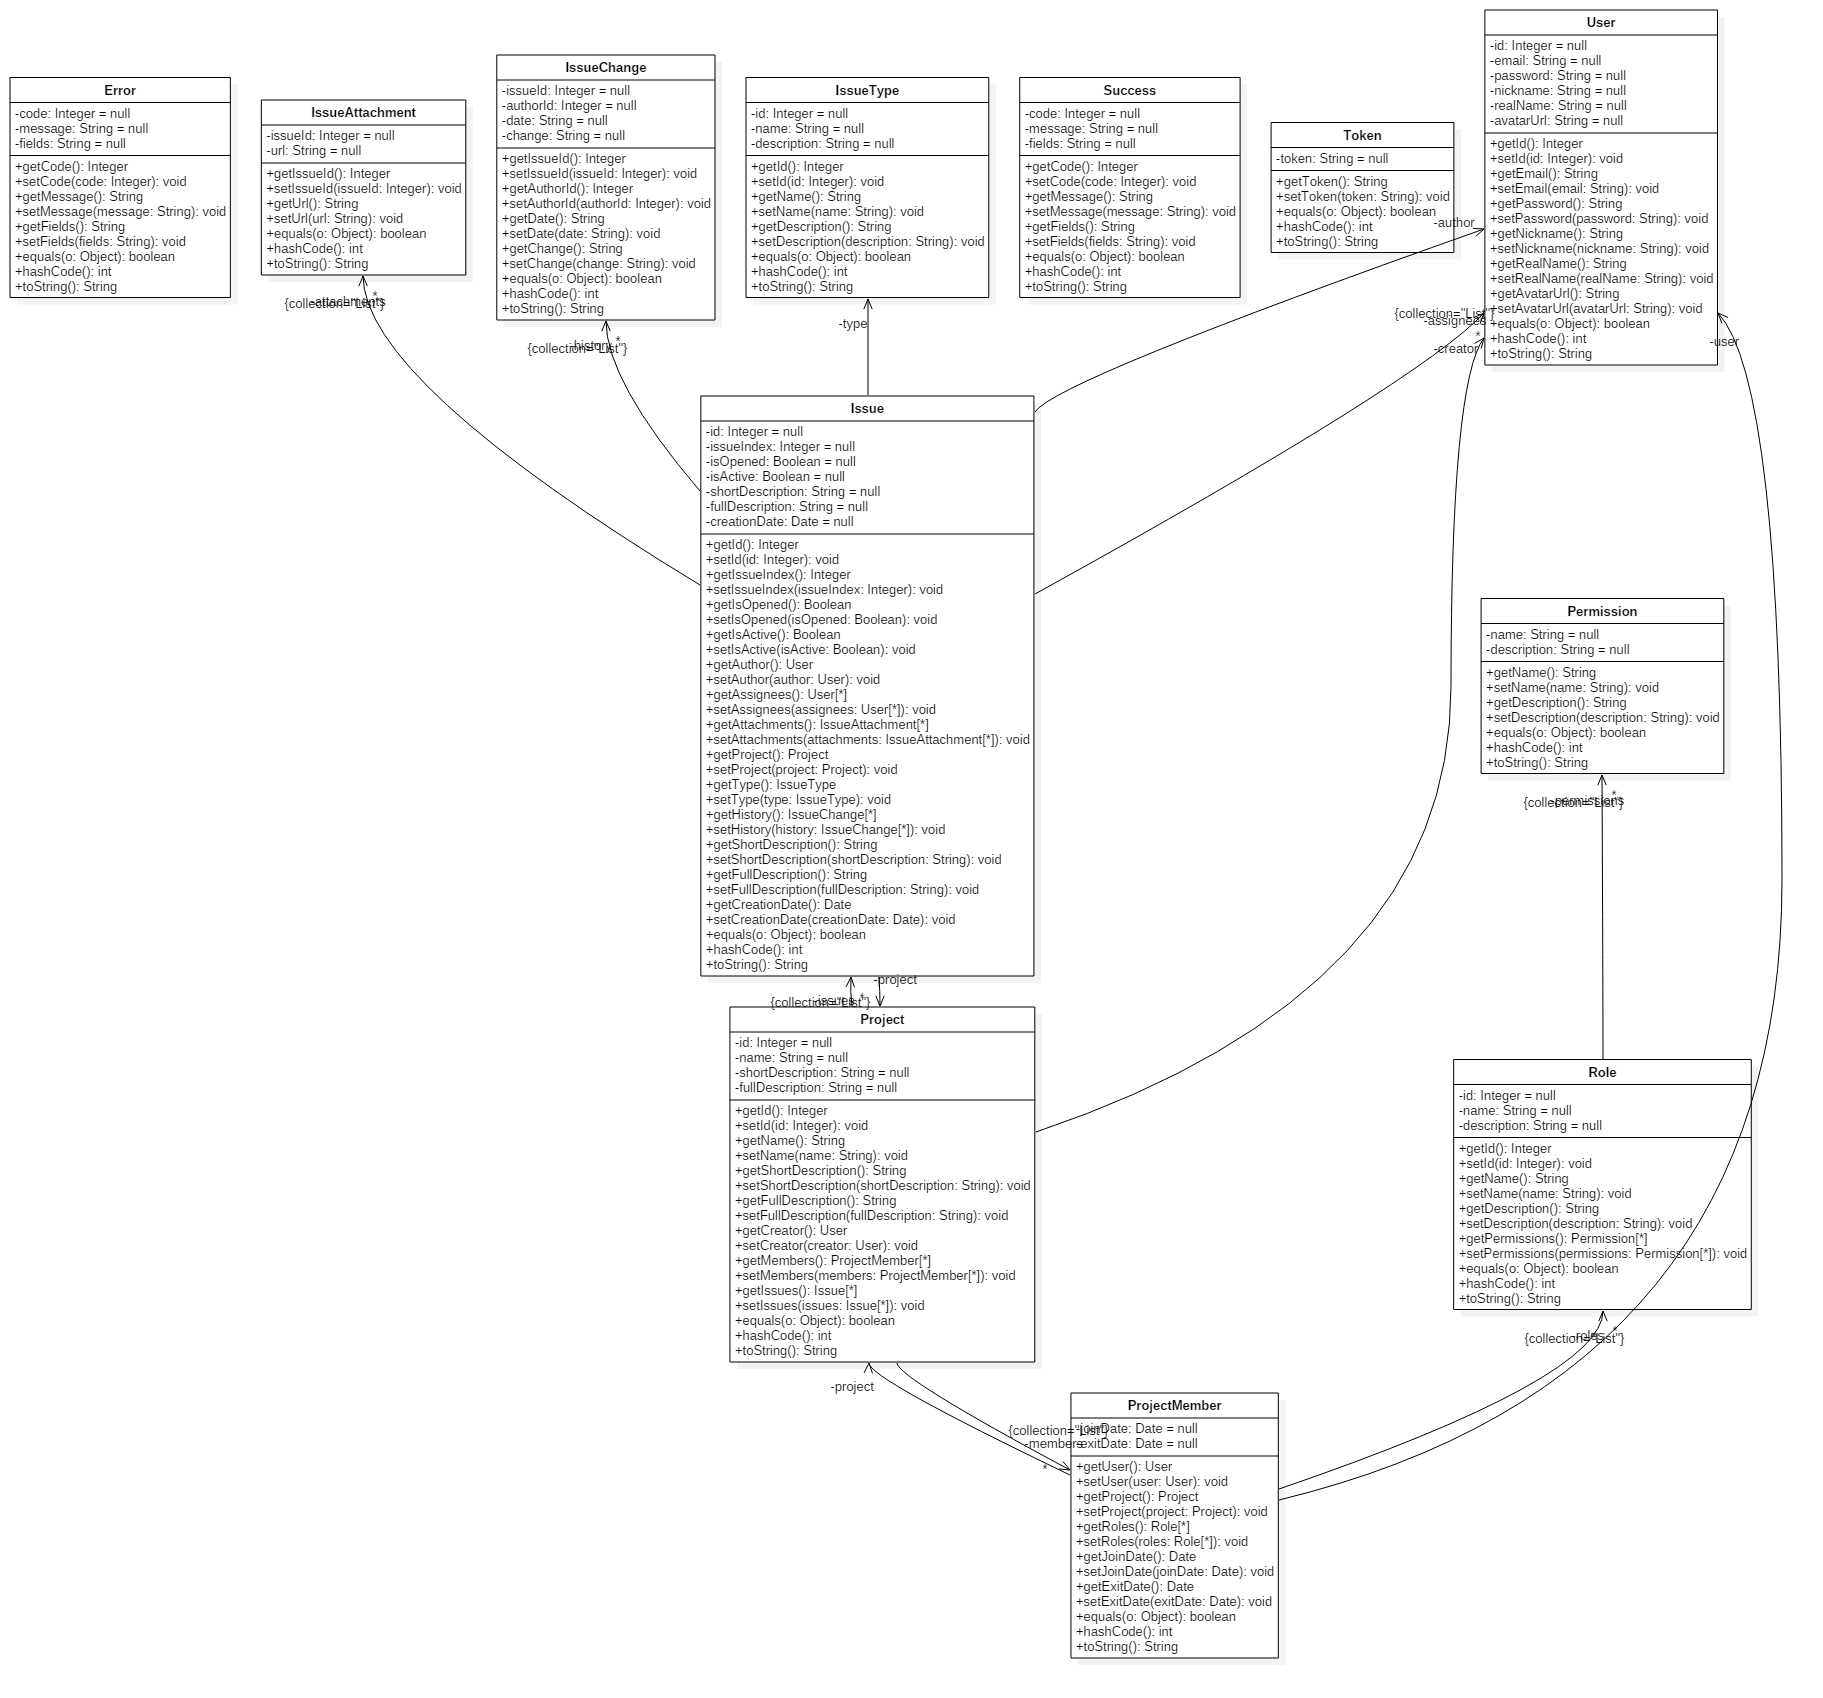
\includegraphics[width=1\textwidth]{3_client_models_diagram}
	\caption{Діаграма моделей даних Android клієнту}
	\label{client_models}
\end{figure}

Для реалізації гнучкої архітектури клієнтського додатку було вирішено використовувати архітектуру, що основується на подіях. На діаграмі \ref{client_events} представлено доступні класи подій Android клієнту.

\begin{figure}[H]
	\centering
	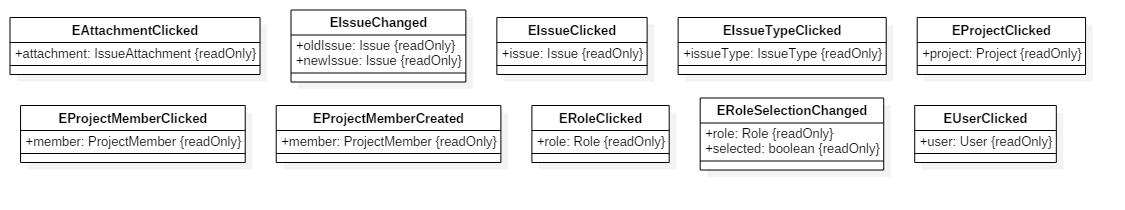
\includegraphics[width=1\textwidth]{3_client_event_classes_diagram}
	\caption{Діаграма класів подій Android клієнту}
	\label{client_events}
\end{figure}

\section{Розгортання програмної системи на апаратних засобах}

Оскільки предметом даної роботи є саме клієнт-серверна система, то розгортання такої системи буде проводитись у декілька етапів:
\begin{enumerate}
	\item Встановлення на серверну машину середовища виконання Node.js.
	\item Забезпечення працездатності серверу бази даних.
	\item Конфігурація серверу.
	\item Розповсюдження клієнтських додатків учасникам системи.
\end{enumerate}

Візуальна демонстрація розгортання системи представлена на рис.~\ref{diagram_deploy}. % to fit all paragraph to one line; otherwise it's either too underfilled or has too short 2nd line

\begin{figure}[H]
	\centering
	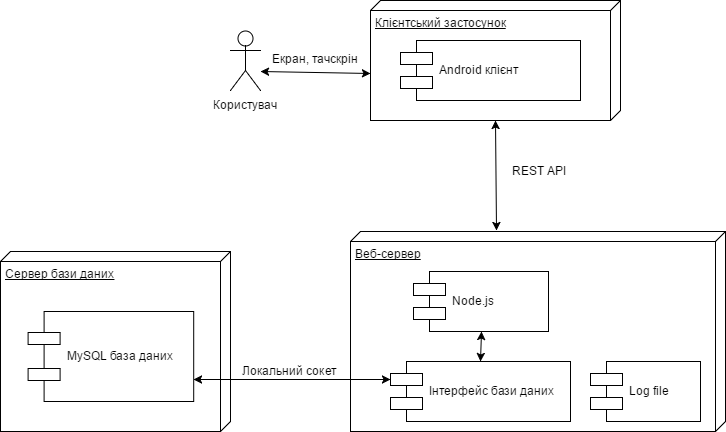
\includegraphics[width=1\textwidth]{3_diagram_deploy}
	\caption{Діаграма розгортання системи}
	\label{diagram_deploy}
\end{figure}

\end{document}